\pgfplotstablegetelem{\thepart}{[index]\columnIndex}\of{\cronograma}
\part{\pgfplotsretval}
\label{part:\thepart}
\frame{\partpage}


\begin{frame}[t]{Exemplos de criação de classe}
	
	\fontsize{14pt}{15}\selectfont{
		
		...continuando.
		
	}\par
	\vspace{1em}
	
	
\end{frame}

\begin{frame}[t]{Atenção}
	\centering
	\begin{tikzpicture}
		%		\node at (0,0){
\includegraphics[width=0.7\textwidth]{imagens/fig-atencao-fundo-branco.png}
			\node (image) 
			{
				
\includegraphics[width=0.7\textwidth]{imagens/fig-atencao-fundo-branco.png}
			};
			\node
			[
			%		fill=teal,
			overlay,
			align=center,
			text=black,
			font={\fontsize{34pt}{19}\bfseries}
			] at (0,-1) (image.center) {Respirem fundo\\ que vamos...};
	\end{tikzpicture}
	
\end{frame}



\begin{frame}[t]{Exemplos de criação de classe}
	
	\lstinputlisting[style=CBruno,caption=Código da classe Produto]{outros/codigos/python/exemplos-de-aulas/src/codigo_003_classe_produto.py}
	
	\vspace{1em}
	
	
\end{frame}


\begin{frame}[t]{Exemplos de criação de classe}	
	
	
	\fontsize{14pt}{15}\selectfont{
		
		Se o código abaixo for colocado junto com o arquivo da classe Produto, é posssível "testar" o código no mesmo arquivo. É desaconselhável fazer.
		
	}\par
	\vspace{1em}
	
	\fontsize{14pt}{25}\selectfont{
		\begin{beamercolorbox}[wd=\textwidth]{warning}
			if \_\_name\_\_ == "\_\_main\_\_":\\
			\hspace{1em}p1 = Produto("Laranja", 1, 1.56, 10)\\
			\hspace{1em}print("Oferta do dia:", p1.obtem\_nome())\\
			\hspace{1em}if p1.altera\_preco(40.00): print("Preco alterado hoje")\\
			\hspace{1em}else: print("Atencao - baixou o preco")
		\end{beamercolorbox}
		
	}\par
	\vspace{1em}
	
\end{frame}




\begin{frame}[t]{Pytest}
	
	\vspace{-2em}
	\lstinputlisting[style=CBruno,caption=Cobertura de testes da classe Produto]{outros/codigos/python/exemplos-de-aulas/tests/test_codigo_003_classe_produto.py}
	
	
	
\end{frame}



\begin{frame}[t]{Pytest}
	
	
	\vspace{1em}
	\centering
	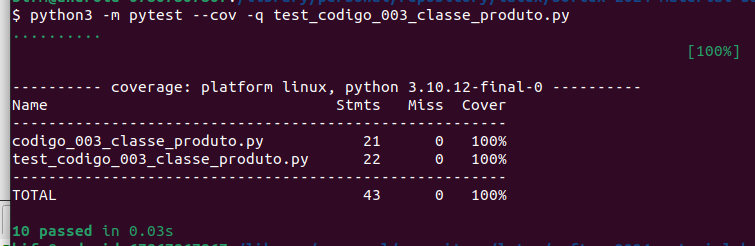
\includegraphics[scale=0.5]{imagens/fig-result-test-class-produto.png}
	
\end{frame}



